%%This is a very basic article template.
%%There is just one section and two subsections.

\documentclass{article}
\usepackage{graphicx}
\begin{document}


\section{480 April 29, 2013 Notes, }

\subsection{QA assignment, it will be posted on April 30, and the same group
will work together again, and using the same bitbucket account}
\textbf{Techniques we will have to use}
\begin{itemize}
  \item Coverage, unit testing, have to cover almost 100 \%, have to find bugs
  too. Can't just cover 100 \% without finding any bugs. Put bugs explanation in
  your reflection.
  \item Code Review.
  \item Wirte Blackbox test,  based on specification completely.
\end{itemize}
\textbf{ What we should not do in this assignment}
\begin{itemize}
  \item We can't have each person do one technique because we all need to know
  this shit.
  \item More communication among team members(bullshit!!!).
\end{itemize}

\textbf{Suggestion}
\begin{itemize}
  \item you splits number of methods.
  \item each apply 3 QA techniques.
\end{itemize}


\subsection{UML diagram}
- We need abstraction to understand big program.\textbf{Definition}: And the
abstraction that we use is UML( stands for Unified Modeling Language), this is a graphical language,
there are 16 UML diagram types\\
- We will learn 4 types:
- UML are blueprint of our program, an abstraction of the program, it tells us
important infomation of the program. For example: blueprint of a building, like
about wireless, electricity, water system diagram\\
- We can apply the same concept, so we can easily track thing in our program
instead of directly looking at the code\\
\begin{itemize}
  \item Strutural vs Behavioral()
  \item Static vs Dynamic( same as static and dynamic analysis)
\end{itemize}

\subsection{Class diagram}
- \textbf{Example}: Class diagram is a static and structural. When people said
draw them a uml diagram, they refer to class diagrams. The look of class diagram is like
the one that we saw when we learnt about class in our 141 class.\\
 - Diagram:\\
  Student--------- name\\
  String name ----- field\\
  int id     ------field\\
  string  name()----- method\\
  - We usually don't even look at the field because they are private, we pay
  more attetion to our methods because they are the ones that we will use.\\

-  There are 3 ways that we can connects class together.
-  \textbf{Connection types in class diagram}
 \begin{itemize}
  \item 1st is \textbf{inheritance}.
  \item 2nd is \textbf{composition}: means own it.
  \item third one we haven't learn is \textbf{agregation}: kinda like
  composition but it is now owning. For example: student can have course but student does not own
  course, but student owns names, ID(composition)
\end{itemize}
\textbf{Note:} The differences between agregation and composition becomes really
important when it comes to C++ because you have to delete your object after you
are done with it, and who deletes whom really matters because you don't want to
forget to delete, or double deletion.
\textbf{Other than connections between classes.}
- You should sometimes use dash arrows for calls, or detects. \\
\pagebreak

\textbf{Figure right here}
\begin{figure}[ht!]
\centering
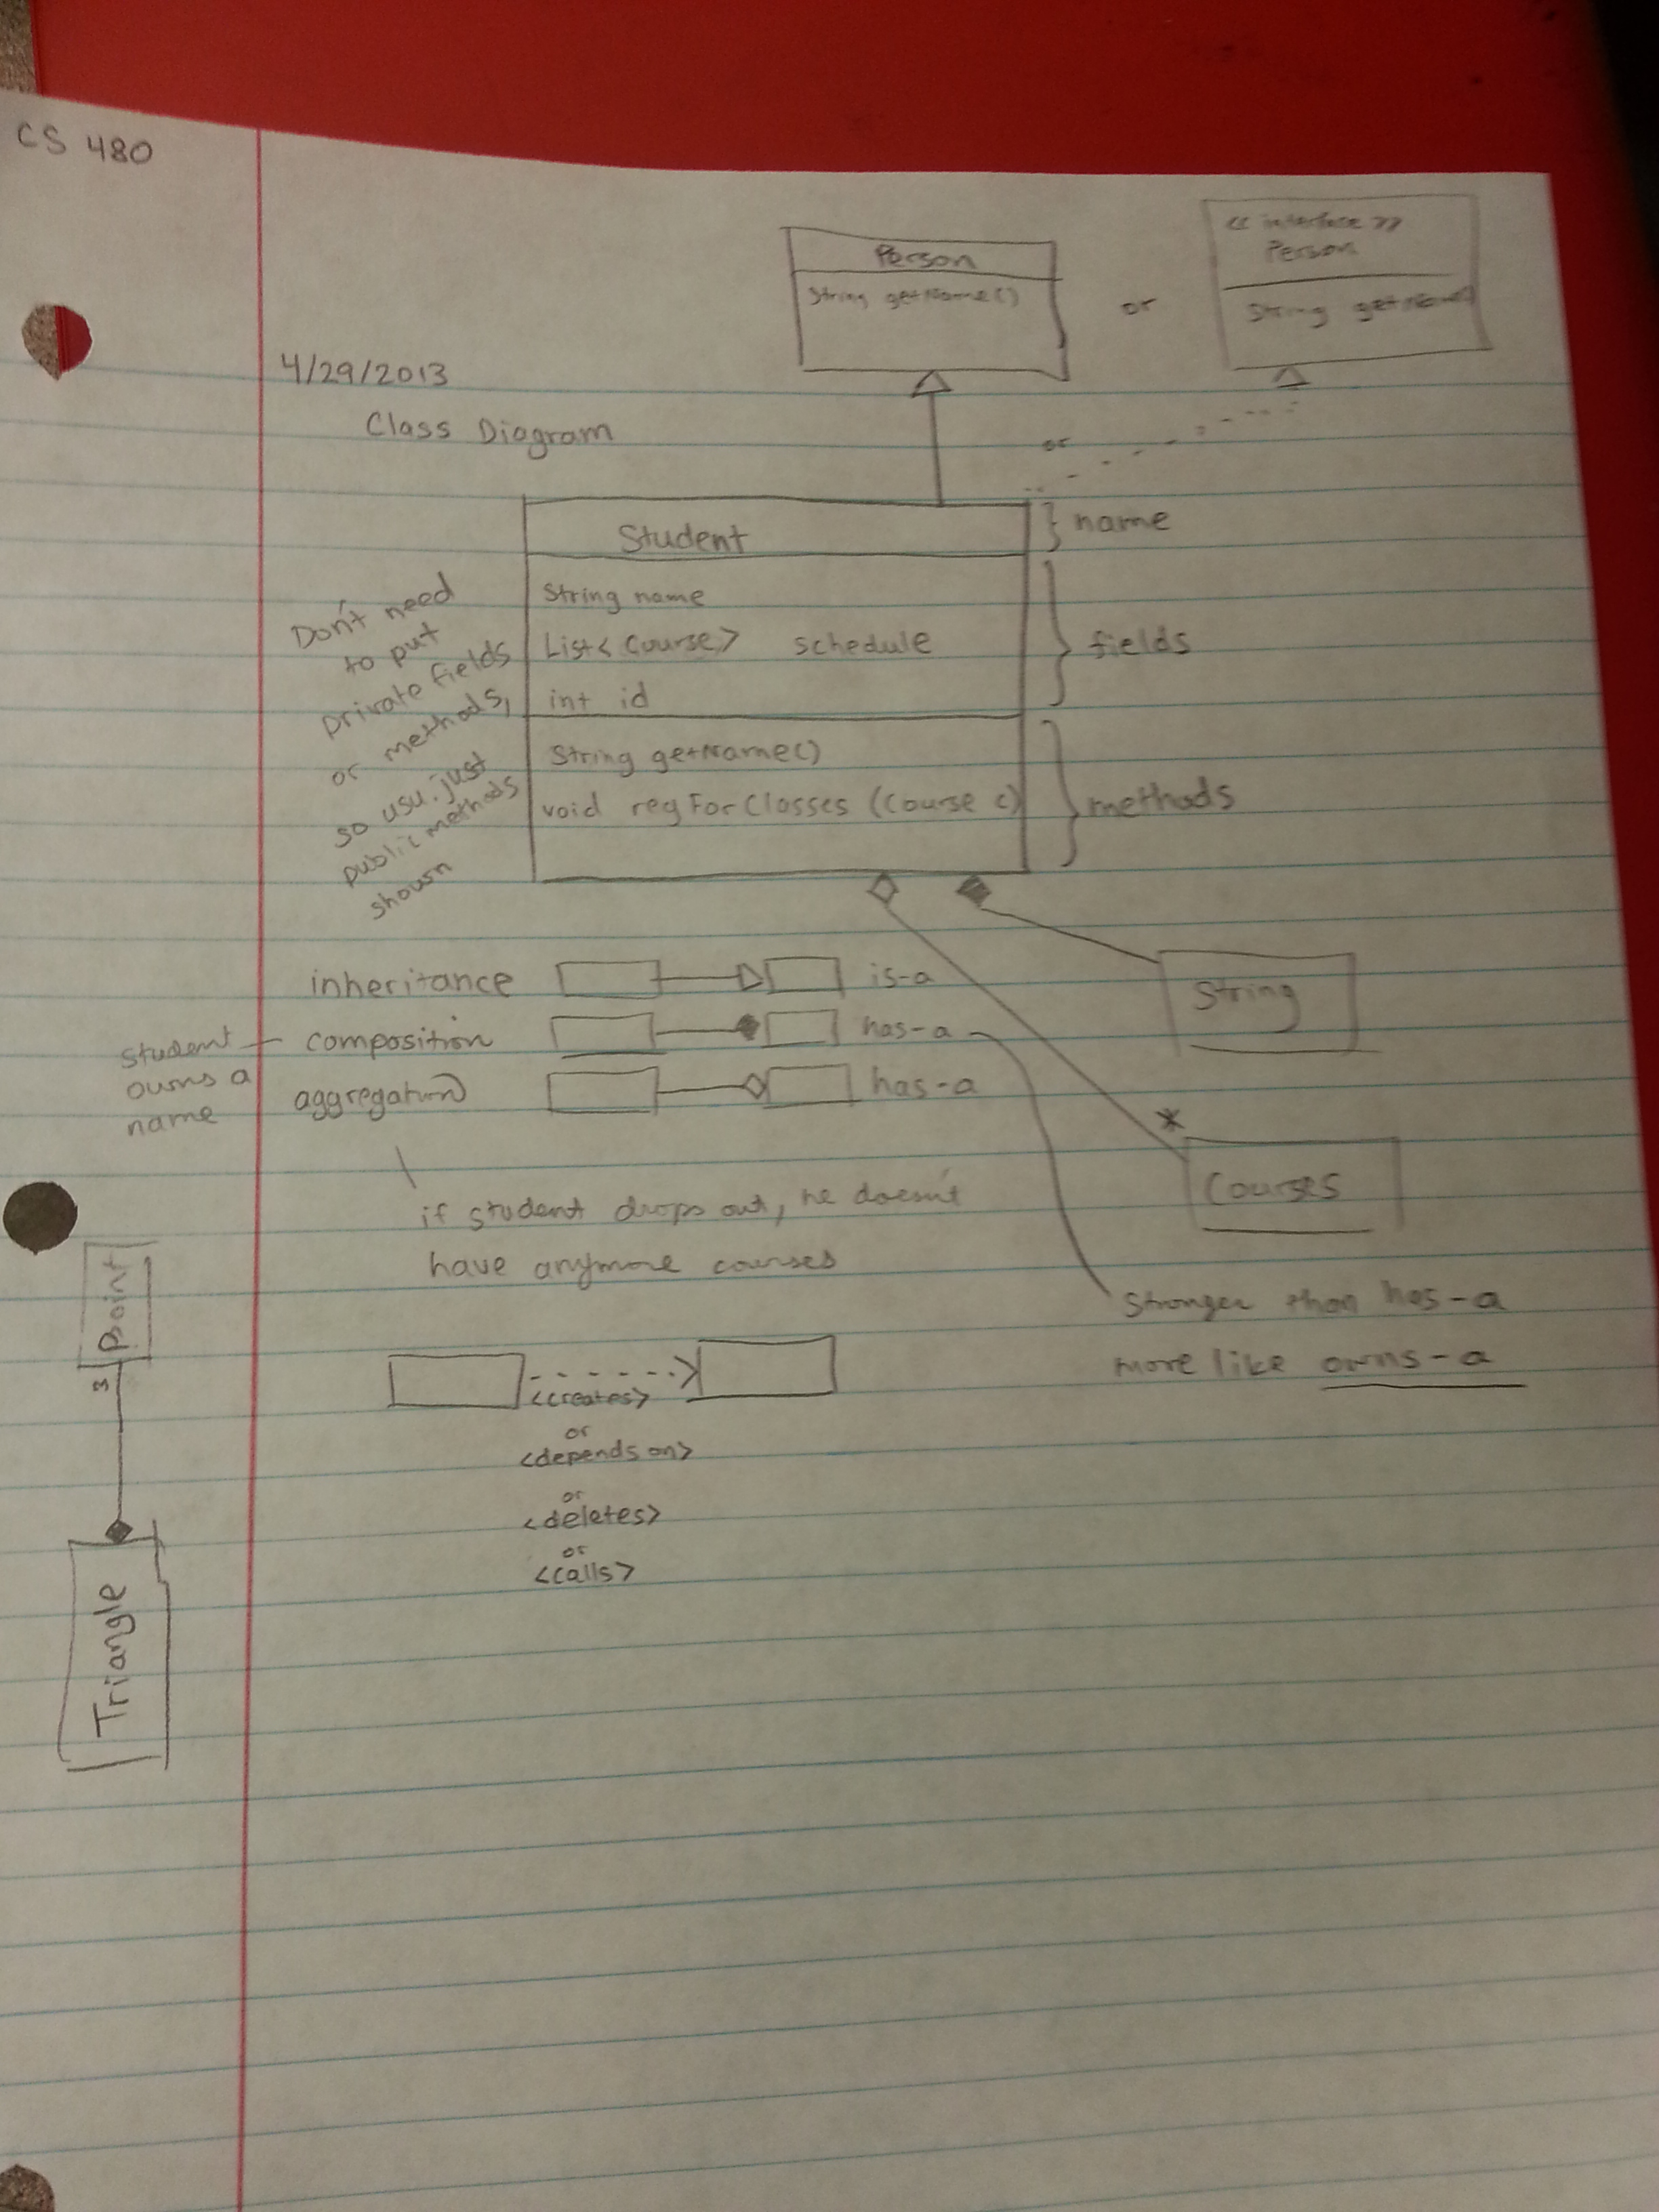
\includegraphics[width=120mm]{figure.jpg}
\caption{Structure Diagram}
\label{overflow}
\end{figure}

\subsection{Object Diagram}
\textbf{Properties}
\begin{itemize}
  \item Dynamic
  \item Structural
\end{itemize}

%picture right here
\textbf{Figure right here}
\begin{figure}[ht!]
\centering
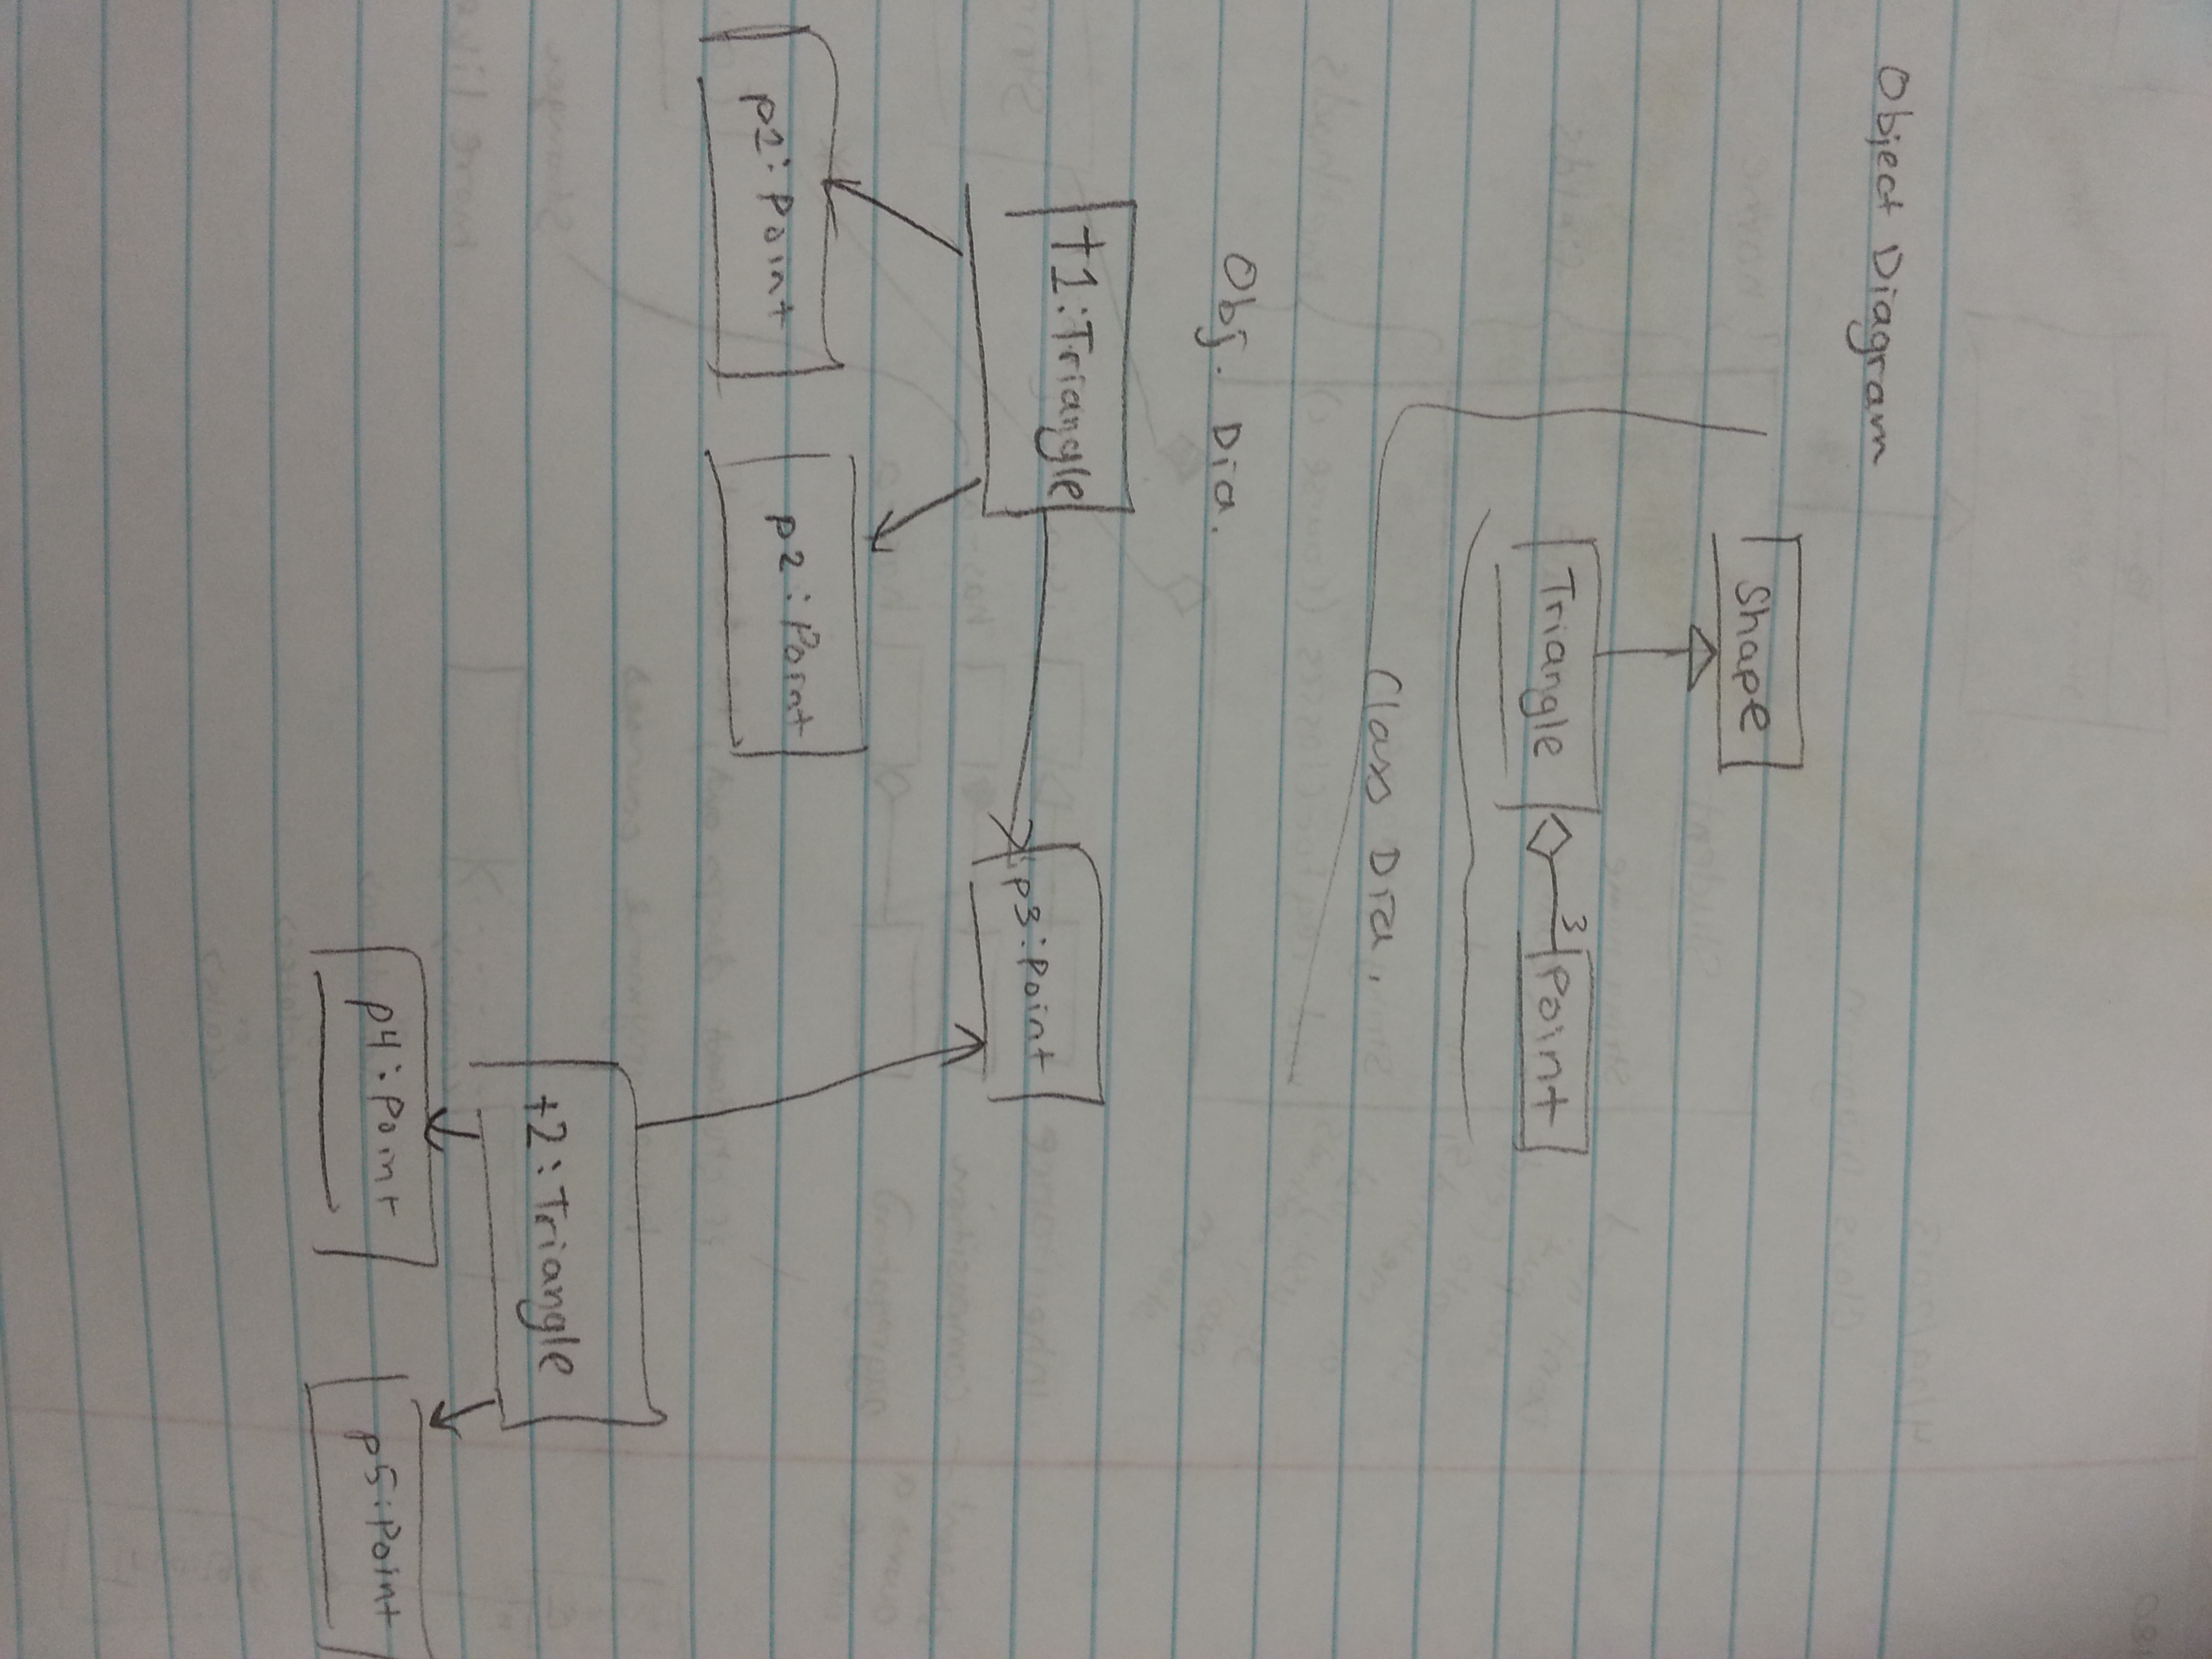
\includegraphics[width=120mm]{figure2.jpg}
\caption{\textbf{Notes:} Object diagram}
\label{overflow}
\end{figure}
\pagebreak

\subsection{Sequence Diagram}
\textbf{Properties}
\begin{itemize}
  \item Dynamic
  \item Behavioral
\end{itemize}


%picture right here
\textbf{Figure right here}
\begin{figure}[ht!]
\centering
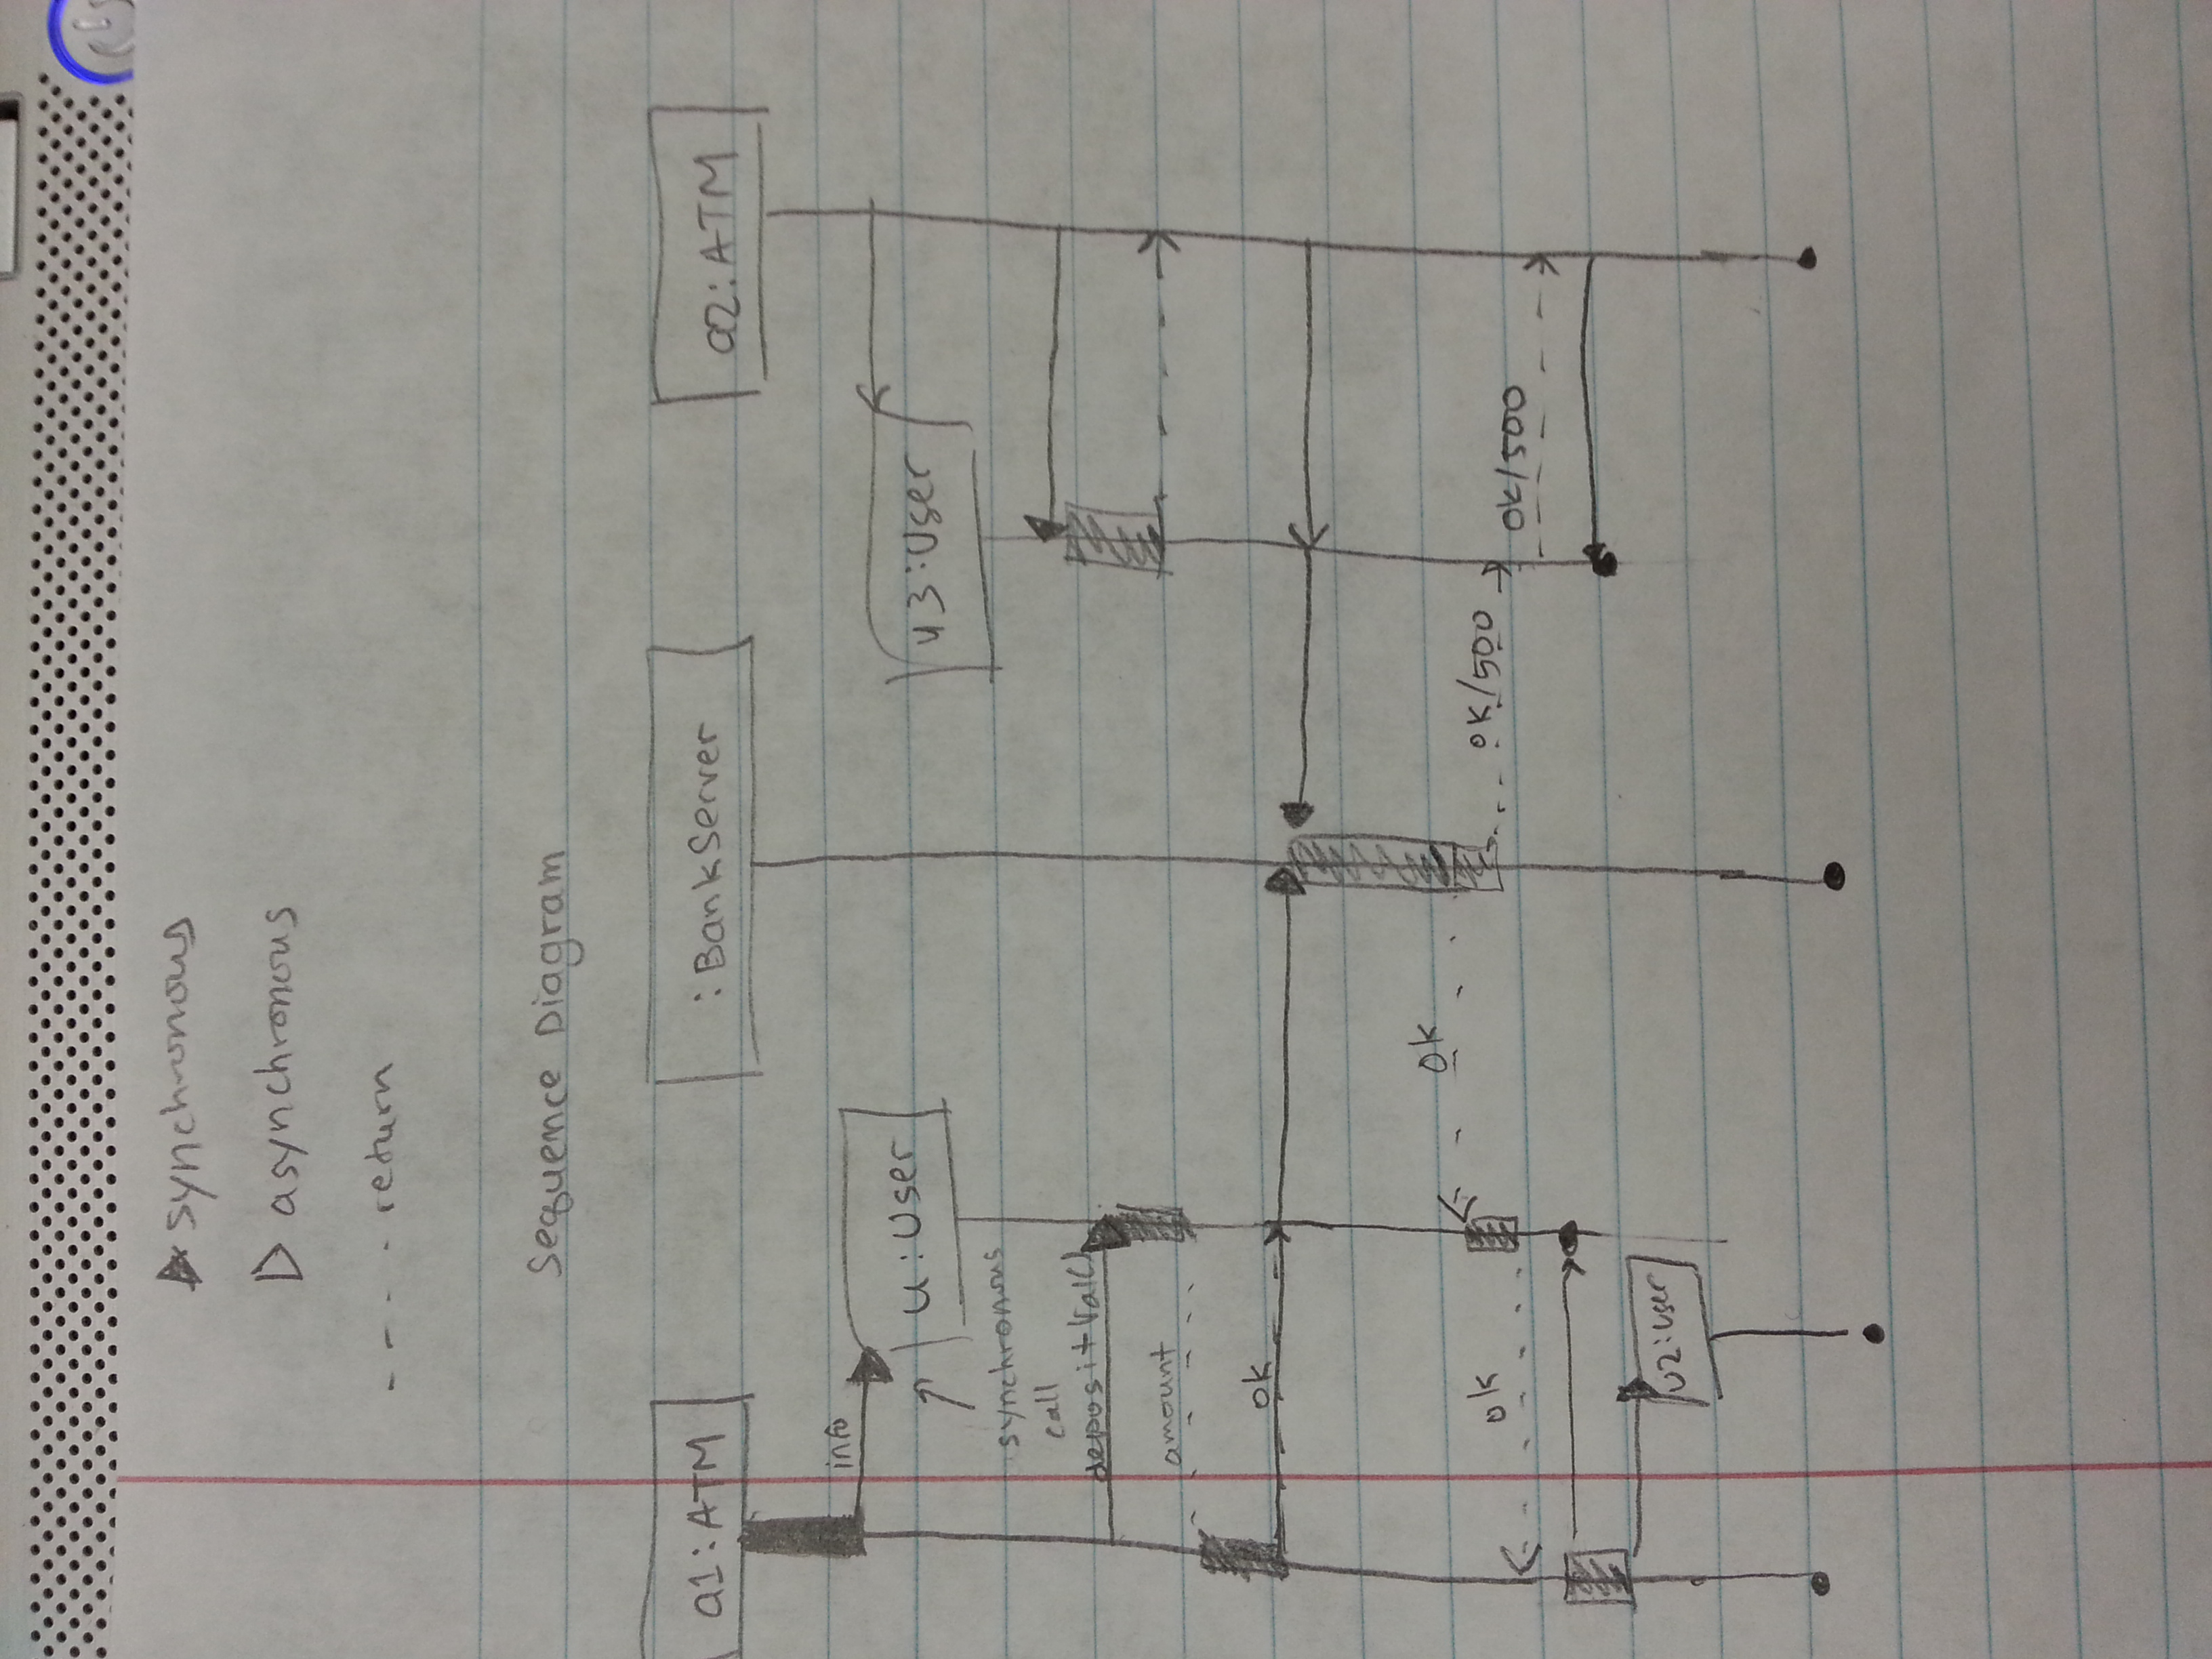
\includegraphics[width=120mm]{figure3.jpg}
\caption{\textbf{Notes:} Dash arrow for returning, solid for giving infomation}
\label{overflow}
\end{figure}
\pagebreak


\subsection{State machine Diagram}
\textbf{Properties}
\begin{itemize}
  \item static
  \item behavioral
\end{itemize}
\textbf{Note:} The diagram of this type looks exactly like automata diagram
\end{document}
